\chapter{Proposed System}

\section{Introduction}
\noindent The proposed system, Vectron, is a distributed vector database designed to store, manage, and retrieve high-dimensional embeddings efficiently while operating on commodity hardware. Unlike conventional vector databases that mandate expensive server-grade infrastructure with substantial memory and compute resources, Vectron achieves efficient resource utilization through intelligent optimizations including int8 quantization, SIMD-accelerated distance computations, and a multi-tier caching architecture.

\noindent Vectron combines Raft-based consensus for strong consistency guarantees, HNSW indexing with performance optimizations, and a microservices architecture to deliver fault-tolerant and scalable performance on modest hardware configurations. The system is implemented in Go using Dragonboat for Raft consensus implementation and a custom HNSW library with SIMD acceleration for distance metric computations.

\\noindent Vectron's primary objective is to democratize vector search by providing a robust, fault-tolerant, and horizontally scalable database system capable of executing on diverse hardware configurations, from legacy commodity machines to modern enterprise servers, while powering semantic search, recommendation engines, and memory components for AI agents.

\section{System Architecture}

The architecture of Vectron is modular, distributed, and service-oriented, following the microservices pattern. The system comprises several interconnected microservices, each performing a specific functional role within the overall architecture.

\noindent The major components of the system are:

\begin{enumerate}
    \item \textbf{API Gateway}
    \begin{enumerate}
        \item Provides REST and gRPC APIs for vector insertion, querying, and collection management.
        \item Applies authentication and rate-limiting middleware for request validation.
        \item Routes requests to appropriate worker nodes through the Placement Driver service.
        \item Implements TinyLFU (Tiny Least Frequently Used) cache algorithm sharded for concurrent access to reduce query latency.
        \item Optionally integrates with Redis/Valkey for distributed caching across API Gateway instances.
        \item Exposes management and monitoring endpoints for cluster observability.
    \end{enumerate}

    \item \textbf{Placement Driver (PD)}
    \begin{enumerate}
        \item Acts as the cluster coordinator utilizing Raft consensus protocol via Dragonboat implementation.
        \item Maintains metadata including collection schemas, shard assignments, and worker node status.
        \item Performs worker node registration and heartbeat processing for health monitoring.
        \item Manages shard assignment and rebalancing operations for load distribution.
        \item Considers failure domain topology for replica placement (rack, zone, region awareness) to maximize fault tolerance.
    \end{enumerate}

    \item \textbf{Worker Nodes}
    \begin{enumerate}
        \item Each worker hosts multiple shard replicas under Raft consensus for strong consistency.
        \item Stores vectors using PebbleDB (a RocksDB-inspired key-value store) for persistent storage.
        \item Implements HNSW-based approximate nearest neighbor search with:
        \begin{itemize}
            \item AVX2/AVX-512 SIMD-accelerated distance computation for vector similarity metrics.
            \item int8 quantization achieving 75\% memory reduction for cosine-normalized vectors.
            \item Two-stage search pipeline with hot index for recent writes and cold mmap-backed index for historical data.
            \item Worker-level search batching for reducing per-request overhead through aggregation.
        \end{itemize}
        \item Supports search-only replicas fed by Write-Ahead Log (WAL) streaming for read scalability.
        \item Processes write operations through Raft proposals ensuring linearizable consistency.
    \end{enumerate}

    \item \textbf{Reranker Service (Optional)}
    \begin{enumerate}
        \item Receives initial search results from worker nodes for post-processing.
        \item Applies rule-based or learning-to-rank strategies for result reordering based on business logic.
        \item Integrates with Redis/Valkey for caching reranking decisions to minimize computation overhead.
        \item Processes user feedback to improve ranking models over time through iterative learning.
    \end{enumerate}

    \item \textbf{Auth Service}
    \begin{enumerate}
        \item Provides JWT (JSON Web Token) based user authentication for secure access control.
        \item Manages API keys for programmatic access and service-to-service authentication.
        \item Stores credentials in etcd (distributed key-value store) for high availability.
        \item Provides a React-based Management Console for cluster monitoring and administration.
    \end{enumerate}

    \item \textbf{Feedback System}
    \begin{enumerate}
        \item Collects user feedback on search results via API Gateway endpoints.
        \item Stores feedback in SQLite for persistence and later analysis.
        \item Enables feedback-driven optimization through the Reranker service.
    \end{enumerate}
\end{enumerate}

\begin{figure} [H]
    \centering
    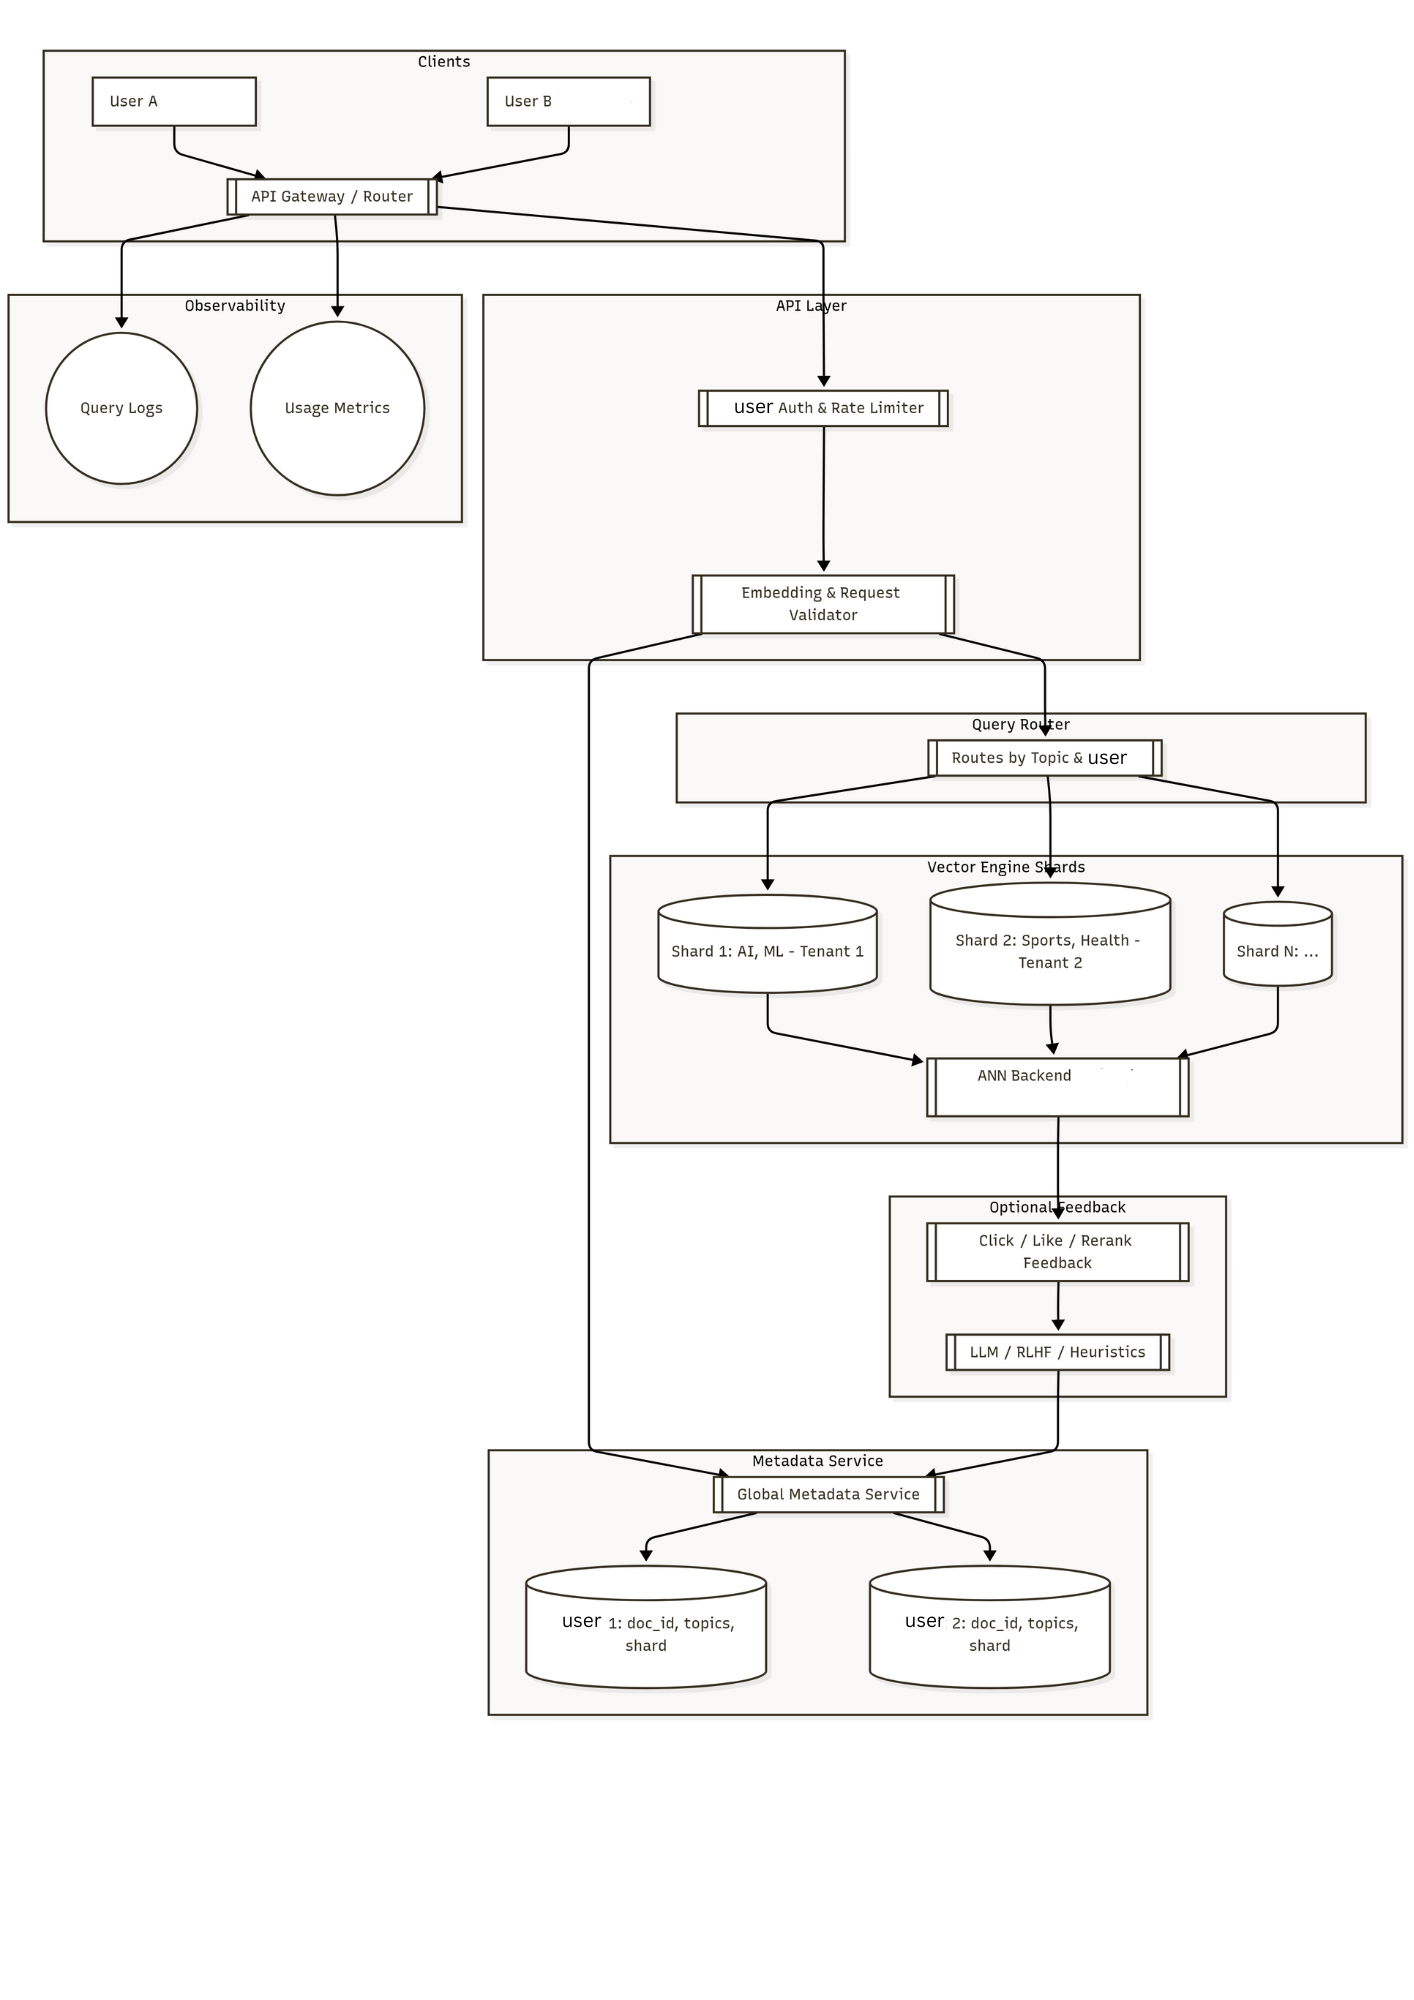
\includegraphics[width=\linewidth]{figures/Images/architecture.png}
    \caption{Proposed System Architecture}
    \label{fig1}
\end{figure}

\section{Data Flow}

The flow of data within Vectron can be divided into four main phases representing the complete lifecycle of vector operations:

\begin{enumerate}
    \item \textbf{Collection Creation Phase}
    \begin{enumerate}
        \item Client invokes CreateCollection operation on API Gateway.
        \item Gateway forwards the request to Placement Driver service.
        \item PD commits collection metadata via Raft consensus and assigns shards to worker nodes.
        \item Result is returned to the client upon successful commit.
    \end{enumerate}

    \item \textbf{Insertion Phase}
    \begin{enumerate}
        \item Client submits vectors through the API Gateway via Upsert operations.
        \item Gateway resolves the target shard and worker node via Placement Driver metadata.
        \item Gateway forwards the upsert request to the appropriate worker node.
        \item Worker proposes the write operation to its Raft group and applies to local state machine.
        \item Vectors are indexed in the hot HNSW index and asynchronously merged to the cold index tier.
    \end{enumerate}

    \item \textbf{Query Phase}
    \begin{enumerate}
        \item The user query is embedded into a vector representation by the client.
        \item Gateway checks TinyLFU cache before forwarding requests to worker nodes.
        \item Gateway resolves candidate worker nodes and shards via Placement Driver metadata cache.
        \item Gateway fans out search RPCs to multiple worker nodes and merges results from distributed shards.
        \item If reranking is enabled, Gateway invokes the Reranker service for post-processing.
        \item Final results are returned to the client after result aggregation.
    \end{enumerate}

    \item \textbf{Feedback Phase}
    \begin{enumerate}
        \item User interactions with search results are collected as implicit feedback signals.
        \item Feedback is persisted in SQLite database via the API Gateway.
        \item The Reranker service leverages feedback data to improve future ranking decisions.
    \end{enumerate}
\end{enumerate}

\section{System Modules}

\begin{table}[h!]
\centering
\begin{tabular}{|l|p{10cm}|}
\hline
\textbf{Module Name} & \textbf{Description} \\
\hline
\textbf{API Gateway} & Unified entry point providing REST/gRPC APIs, TinyLFU caching, optional Redis/Valkey integration, authentication/rate-limiting middleware, and request routing to worker nodes. \\
\hline
\textbf{Placement Driver} & Cluster coordinator with Raft consensus (via Dragonboat) for metadata management, shard assignment, worker health monitoring, and failure-domain-aware replica placement. \\
\hline
\textbf{Worker Nodes} & Data nodes utilizing PebbleDB storage, HNSW indexing with SIMD acceleration and int8 quantization, hot/cold index tiering, and per-shard Raft replication for strong consistency. \\
\hline
\textbf{Reranker Service} & Applies rule-based or machine learning strategies to reorder search results with Redis/Valkey caching for reduced latency. \\
\hline
\textbf{Auth Service} & JWT-based authentication, API key management, etcd-backed storage for high availability, and React-based Management Console for monitoring. \\
\hline
\textbf{Feedback System} & Collects and persists user feedback in SQLite for continuous retrieval quality improvement. \\
\hline
\end{tabular}
\caption{System Modules and Their Descriptions}
\end{table}

\vspace{2cm}
\section{Algorithms and Technologies Used}
\begin{enumerate}
    \item \textbf{HNSW (Hierarchical Navigable Small World)}
    \begin{itemize}
        \item Graph-based ANN algorithm constructing multi-layer proximity graphs for efficient similarity search.
        \item Provides logarithmic search complexity with high recall at low latency.
        \item Custom Go implementation with memory-mapped (mmap) vector storage for efficient memory utilization.
    \end{itemize}

    \item \textbf{SIMD Acceleration (AVX2/AVX-512)}
    \begin{itemize}
        \item AVX2-accelerated distance computation for float32 vectors using 256-bit vector registers.
        \item AVX-512-accelerated dot product operations for int8 quantized vectors using 512-bit vector registers.
        \item Runtime CPU feature detection for automatic dispatch to optimal code path (AVX-512, AVX2, or scalar fallback).
    \end{itemize}

    \item \textbf{int8 Quantization}
    \begin{itemize}
        \item Converts float32 vectors to int8 representations achieving 75\% memory reduction (4 bytes to 1 byte per dimension).
        \item Applicable exclusively for cosine-normalized vectors where the L2 norm equals 1.
        \item SIMD-accelerated quantization using AVX2 instructions for fast conversion.
    \end{itemize}

    \item \textbf{Raft Consensus Protocol (Dragonboat)}
    \begin{itemize}
        \item Ensures strong consistency across distributed worker nodes through majority quorum replication.
        \item Handles leader election, log replication, and safety properties for fault tolerance.
        \item Utilized for both Placement Driver metadata store and per-shard vector data replication.
    \end{itemize}

    \item \textbf{PebbleDB Storage}
    \begin{itemize}
        \item Key-value storage engine serving as the persistence layer for vector data and metadata.
        \item Provides efficient read/write operations with automatic compaction for garbage collection.
    \end{itemize}

    \item \textbf{Multi-Tier Caching Architecture}
    \begin{itemize}
        \item Gateway-level TinyLFU cache sharded across goroutines for concurrent access.
        \item Optional distributed Redis/Valkey cache for cross-instance cache sharing.
        \item Worker-local search result caches for minimizing redundant ANN computations.
    \end{itemize}
\end{enumerate}

\section{Features of the Proposed System}
\begin{itemize}
    \item \textbf{Commodity Hardware Support:} Optimized for execution on modest hardware through int8 quantization and SIMD acceleration, reducing memory footprint and CPU cycles required.
    \item \textbf{Strong Consistency:} Raft-based replication ensures linearizable consistency across distributed nodes.
    \item \textbf{Low-Latency Search:} HNSW indexing with SIMD provides sub-10ms approximate nearest neighbor queries.
    \item \textbf{Memory Efficiency:} int8 quantization reduces memory requirements by 75\% compared to float32 storage.
    \item \textbf{Fault Tolerance:} Multi-Raft shard replicas with automatic failover and leader re-election.
    \item \textbf{Feedback Integration:} User feedback collection mechanism for continuous ranking improvement.
    \item \textbf{Horizontal Scalability:} Worker node addition increases system capacity through shard redistribution.
    \item \textbf{Management Console:} React-based dashboard for cluster monitoring and administrative operations.
\end{itemize}

\section{Advantages}
\begin{enumerate}
    \item Executes efficiently on older commodity hardware without performance degradation.
    \item Strong consistency guarantees through Raft consensus applied to both metadata and data operations.
    \item Efficient vector search through optimized HNSW indexing with logarithmic time complexity.
    \item 75\% memory reduction through int8 quantization enabling larger datasets on limited hardware.
    \item SIMD acceleration improving throughput on compatible hardware through vectorized operations.
    \item Improved retrieval quality through feedback-driven reranking using rule-based strategies.
    \item Secure multi-tenant access control with JWT tokens and API key authentication.
    \item Robust fault tolerance with per-shard Raft replication and automatic failover mechanisms.
    \item Horizontally scalable architecture supporting linear throughput growth with additional worker nodes.
    \item Comprehensive monitoring and management capabilities through integrated dashboard.
\end{enumerate}

\section{Summary}
The proposed system, Vectron, integrates advanced vector search algorithms with distributed microservices architecture and commodity-hardware-first optimization strategies. It provides a robust framework for semantic retrieval that supports fault tolerance, horizontal scalability, and efficient operation on modest hardware configurations. Through int8 quantization (reducing per-vector storage from 4 bytes to 1 byte), SIMD acceleration (utilizing AVX2/AVX-512 instructions), and multi-tier caching (TinyLFU at gateway, Redis/Valkey distributed, worker-local), Vectron democratizes vector search by making it accessible to organizations without enterprise infrastructure budgets. This system bridges the gap between enterprise-grade vector databases and accessible hardware platforms, forming the foundation for future large-scale, cost-effective retrieval engines capable of operating on heterogeneous hardware.